% !TEX program = xelatex
\documentclass[11pt,a4paper]{article}

\usepackage[margin=2.5cm,headheight=14pt]{geometry}
\usepackage{fontspec}
\usepackage{xeCJK}
\setmainfont{Times New Roman}
\setsansfont{Arial}
\setmonofont{Consolas}
\setCJKmainfont{SimSun}
\setCJKsansfont{Microsoft YaHei}
\setCJKmonofont{SimSun}

\usepackage{amsmath,amssymb}
\usepackage{booktabs}
\usepackage{multirow}
\usepackage{graphicx}
\usepackage{caption}
\usepackage{subcaption}
\usepackage{enumitem}
\usepackage{xcolor}
\usepackage{microtype}
\usepackage{fancyhdr}
\usepackage{titlesec}
\usepackage{natbib}
\usepackage{siunitx}
\usepackage{setspace}
\usepackage{hyperref}
\usepackage{url}
\usepackage{float}
\usepackage{tikz}
\usetikzlibrary{arrows.meta,positioning,calc}

\hypersetup{colorlinks=true,linkcolor=blue!60!black,citecolor=blue!60!black,urlcolor=blue!60!black}

\captionsetup{font=small,labelfont=bf}
\setlength{\tabcolsep}{5pt}
\renewcommand{\arraystretch}{1.15}
\setstretch{1.08}

\pagestyle{fancy}
\fancyhf{}
\fancyhead[L]{\small\itshape Weakly-Supervised Chinese Review Sentiment Classification}
\fancyhead[R]{\small\thepage}
\renewcommand{\headrulewidth}{0.4pt}

\titleformat{\section}{\large\bfseries}{\thesection}{0.8em}{}
\titleformat{\subsection}{\normalsize\bfseries}{\thesubsection}{0.8em}{}
\titleformat{\subsubsection}{\normalsize\itshape}{\thesubsubsection}{0.8em}{}
\setlist[itemize]{leftmargin=1.5em,itemsep=2pt,topsep=3pt}
\setlist[enumerate]{leftmargin=1.5em,itemsep=2pt,topsep=3pt}

\newcommand{\code}[1]{\texttt{#1}}

\begin{document}

%=====================================================================
\begin{titlepage}
\thispagestyle{empty}
\begin{center}
\vspace*{2.0cm}
{\LARGE\bfseries Weakly-Supervised Chinese Review Sentiment\\[6pt]
Classification at Scale:\\[6pt]
Pseudo-Labeling, Specialist Decomposition,\\[6pt]
and Honest Out-of-Distribution Evaluation}\par
\vspace{0.9cm}
{\large\itshape Undergraduate Thesis --- Natural Language Processing}
\par
\vspace{2.6cm}
\begin{tabular}{ll}
\textbf{Student}    & Shuakami \\
\textbf{Date}       & \today \\
\end{tabular}
\vfill
{\footnotesize\itshape
Code, out-of-fold predictions, and full experiment records:
\url{https://github.com/shuakami/douban-sentiment}}
\end{center}
\end{titlepage}

%=====================================================================
\begin{abstract}
\begingroup
\small
\noindent
We study three-class sentiment classification (positive / neutral /
negative) of Chinese Douban movie short reviews under a realistic
low-resource setting: 600 human-verified semantic labels plus a large
weakly-labelled corpus of 910{,}998 reviews with star ratings. Our study
makes four contributions. First, we \emph{measure} that star ratings are
a poor proxy for semantic sentiment: on a 271{,}905-row confident
pseudo-label pool, only $\sim$59\% of 5-star reviews are predicted
positive, and 3-star reviews skew negative rather than neutral.
Second, we show that pseudo-labelling the corpus with a distilled
ensemble and training a single compact student on 160K balanced rows
reaches 87.5\% accuracy with 84.8\% neutral recall on the gold set ---
evidence that label quality at scale, not model capacity, is the binding
constraint. Third, our deployed system couples a distilled MacBERT
student, a frozen MegatronBERT-1.3B feature judge, and a
corpus-trained neutral specialist, reaching \textbf{89.5\% accuracy /
85.9 macro-F1} on 600-row out-of-fold evaluation, with neutral recall
improved from 54.3\% to 70.7\%. Fourth, we construct \textbf{lab2000},
a 2{,}000-row cross-movie benchmark with two-pass LLM blind
annotation (same annotator model, different few-shot views) and
479 human-adjudicated rows, and show that the gold-trained system
generalises poorly to wild short reviews (65.0\% three-class) --- but
that adding only 1{,}000 actively-selected boundary examples lifts the
SFT student by $+8.8$pp (62.6\%$\to$71.4\%, McNemar
$p = 4.0\times10^{-8}$).
Scaling the same protocol with frontier-LLM pseudo-labels --- up to
$\sim$17K actively-selected examples --- pushes the ensemble mix to
\textbf{77.1\% three-class} (74.6--76.3\% across five seeds,
77.1\% seed-averaged by averaging the seeds' probability outputs
before decoding; 5-fold cross-fit validated; significantly above
the 1K-AL mix, McNemar $p = 3.9\times10^{-4}$), above the measured 71.5\%
second-annotator agreement reference, and lifts
binary OOD to \textbf{92.3\%}. We
further report three empirical observations invisible at $n{=}600$:
active-learning
samples require a gold anchor to avoid prior collapse, hard labels may
beat soft distillation under domain shift, and star ratings become the
strongest signal precisely where text is most ambiguous. All negative
results --- more than twenty rejected architectures --- are documented.
\par\endgroup
\end{abstract}

\vspace{0.6em}
\noindent{\small\itshape\textbf{Keywords:} sentiment analysis;
Chinese NLP; weak supervision; pseudo-labelling; knowledge
distillation; pre-trained language models; calibration;
out-of-distribution evaluation.}

\newpage
\tableofcontents
\newpage

%=====================================================================
\section{Introduction}
\label{sec:intro}

Short reviews on Douban --- China's most influential movie community ---
are terse, ironic, and frequently mix praise with criticism. A typical
review reads \emph{``特效无敌，但是剧情简直像一坨''} (``the special
effects are unbeatable, but the plot is literally a pile of trash'').
Such mixed-polarity text is precisely where three-class sentiment
analysis (positive / neutral / negative) breaks down: the neutral class
is both the most frequent source of ambiguity and the hardest to learn
from few examples.

This project addresses a realistic low-resource scenario: a course
assignment provides 600 reviews with human-verified semantic labels,
while the platform additionally offers a corpus of nearly one million
Douban comments carrying only star ratings (1--5). Two research questions
organize the work:

\begin{enumerate}
  \item \textbf{RQ1.} Can a small labelled set be amplified by a large
        weakly-labelled corpus?
  \item \textbf{RQ2.} Can specialist decomposition --- a dedicated
        neutral expert trained on corpus-scale pseudo-labels --- repair
        the weakest class without degrading the rest?
\end{enumerate}

Our answer is yes to both, but with an important honest caveat: the
corpus amplifies \emph{coverage}, not \emph{knowledge}. Pseudo-labels are
produced by our own models, so the flywheel saturates after one round;
the true bottleneck is annotation noise on terse comments, which we
quantify with a dedicated out-of-distribution study.

\paragraph{Contributions.}
\begin{itemize}
  \item A measured analysis showing star ratings are unreliable weak
        supervision for three-class sentiment (corpus-wide three-class
        agreement between pseudo-labels and ratings $\approx$48\%).
  \item A pseudo-label flywheel producing a 271{,}905-row confident pool
        and a single compact student (87.5\% acc / 84.8\% neutral recall)
        trained with no gold labels in its training set.
  \item A deployed hybrid ensemble (89.5\% acc / 85.9 macro-F1,
        neutral recall 70.7\%) combining a distilled student, a frozen
        1.3B-parameter judge, and a corpus-trained neutral specialist.
  \item A reproducible evaluation protocol (stratified 5-fold OOF,
        cross-fit fusion-weight selection, McNemar/bootstrap
        significance tests, temperature calibration)
        plus a 2{,}000-row cross-movie benchmark (lab2000) under which
        active-learning expansion adds +8.8pp over gold-only SFT
        ($p \approx 4\times10^{-8}$) and scaling to 17K LLM labels
        reaches 77.1\% three-class accuracy --- above the measured
        71.5\% second-annotator agreement reference.
  \item A documented catalogue of more than twenty measured-but-rejected
        architectures, which we argue is itself a contribution: it maps
        the effective design space for this task.
\end{itemize}

%=====================================================================
\section{Related Work}
\label{sec:related}

\paragraph{Sentiment analysis of Chinese text.}
Document-level sentiment classification has a long history, from
feature-based methods (unigrams, character $n$-grams) to neural
architectures \citep{kim2014,socher2013,joulin2017,reimers2019};
comprehensive surveys are given by \citet{pang2008} and, for Chinese
specifically, by \citet{tan2008}. For Chinese, the absence of
whitespace tokenization makes character-level features and pretrained
language models especially effective. Douban reviews specifically have
been used in earlier Chinese sentiment work --- including weak-label
pipelines combining dictionaries with rating-derived supervision
\citep{fan2018} --- but almost exclusively as
a binary (positive/negative) task; the three-class setting with a
genuine neutral/mixed class is less studied and substantially harder.
The difficulty of the neutral/mixed class is documented for
document-level polarity classification more broadly
\citep{martins2021}.

\paragraph{Pre-trained language models.}
BERT \citep{devlin2019} and its robustly-optimised successor RoBERTa
\citep{liu2019} established the pretrain-then-finetune paradigm. For
Chinese, MacBERT \citep{cui2020} replaces the MLM objective with a
corrected variant better suited to character-level inputs, ERNIE
\citep{sun2019} integrates entity and phrase knowledge, while
StructBERT \citep{wang2020} injects phrase- and word-level structural
information into pre-training. Erlangshen-MegatronBERT
\citep{idea2023} scales this family to 1.3B parameters with additional
sentiment fine-tuning. We use all three families and compare
them directly.

\paragraph{Weak supervision and self-training.}
When labelled data is scarce, distant supervision from noisy signals
(star ratings here) and self-training on model predictions are standard
remedies \citep{yarowsky1995,lee2013}. The Snorkel framework
\citep{ratner2017} and the WRENCH benchmark \citep{zhang2021wrench}
formalise the combination of multiple weak label
sources. The gap between star ratings and textual sentiment is itself
long documented --- ratings were already treated as imperfect proxies
in early work \citep{pang2005seeing} and rating--sentiment
incongruence has been measured directly on review corpora
\citep{abaiyan2026stars}. Active learning \citep{settles2009} instead spends a small
annotation budget on the most informative examples; our Stage-2 study
uses margin/entropy sampling for exactly this purpose. Our work
differs in that we \emph{measure} the weakness of the
dominant weak source (ratings) before relying on it, and we quantify
where pseudo-labelling helps (neutral coverage) versus where it cannot
(helping beyond the teacher's knowledge).

\paragraph{Knowledge distillation.}
Hinton et al.'s dark-knowledge distillation \citep{hinton2015}
--- surveyed comprehensively by \citet{gou2021} --- lets a
small student mimic a large teacher's soft predictions. We distil a
7-channel teacher ensemble into a single MacBERT-base student and
validate every ensemble decision with out-of-fold predictions.
Knowledge distillation under distribution shift is itself an active
research area \citep{zhang2023shiftkd}; our hard-vs-soft comparison
in Section~\ref{sec:findings} is a small-scale instance of the same
question.

\paragraph{Calibration.}
Neural classifiers are systematically over- or under-confident
\citep{guo2017}. We apply temperature scaling --- a single-parameter
post-hoc fix --- and report expected calibration error before and
after, because honest confidence display matters for a demo system.

\paragraph{LLMs as annotators and baselines.}
General-purpose LLMs are increasingly used for zero-/few-shot
classification \citep{gilardi2023,tornberg2023}, for generating
synthetic training data, and as annotators whose agreement with human
labels is known to overstate quality on subjective tasks
\citep{moller2024parrot,schroeder2025}. We evaluate
Qwen3 models \citep{qwen2025} at 0.6B/1.7B/4B scales both as zero-shot
classifiers and as independent annotators in our OOD study, and we
report a negative result on LLM-generated synthetic augmentation.

%=====================================================================
\section{Task and Datasets}
\label{sec:data}

\subsection{Task definition}

Given a Douban movie short review $x$, predict
$y \in \{\text{positive}, \text{neutral}, \text{negative}\}$. These
reviews tend to be brief --- the corpus median is only 24 characters
--- and a single line often mixes sarcasm, allusions to a specific
film, and conflicting evaluations. We count as neutral those reviews
that carry no clear polarity: bare plot summaries, evenly balanced
praise and criticism, and meta-commentary such as ``seen it, no
comment''. Table~\ref{tab:examples} shows representative cases,
including the mixed-polarity pattern that dominates the error
analysis.

\begin{table}[H]
\centering\small
\caption{Representative gold-set reviews (Chinese original with English
gloss). ``Mixed$\to$Neg'' denotes a praise-then-criticism review whose
final polarity is negative.}
\label{tab:examples}
\begin{tabular}{p{5.6cm}p{5.4cm}cl}
\toprule
Review & Gloss & Label & Len \\
\midrule
``特效无敌，但是剧情简直像一坨。'' & Effects unbeatable, plot a
pile of trash & Neg & 15 \\
``演技、镜头、配乐都是顶级，现代经典。'' & Acting, camera, score all
top-tier; modern classic & Pos & 18 \\
``看在演员的份上值回票价，剧情很套路。'' & Worth it for the cast;
routine plot & Neu & 17 \\
``两个小时的生命浪费，想喜欢它都难。'' & Two hours wasted; hard to
like & Neg & 17 \\
``又是续集，还行吧。'' & Another sequel; it's okay & Neu & 9 \\
\bottomrule
\end{tabular}
\end{table}

\subsection{Gold set (600 reviews)}

The labelled evaluation set contains 600 reviews sampled from a single
film page, each annotated with \code{label\_semantic} (human-verified
semantic sentiment) and \code{label\_rule} (star-derived weak label).
Class distribution: 316 positive / 92 neutral / 192 negative.
Reviews are comparatively long (mean 110.8, median 80 characters).
The neutral class is supported by only 92 examples --- the smallest
and hardest class.

\subsection{Weakly-labelled corpus (910{,}998 reviews)}

The Moviedata-10M corpus \citep{douban2024} --- 4{,}428{,}475 raw Douban
comments --- yields 910{,}998 cleaned, deduplicated comments after our own
cleaning, across 20{,}966 films and 249{,}105 users, with
star rating
(1--5), timestamp, and vote counts but \emph{no} semantic labels.
Review length: mean 40.6 / median 24 / p90 = 102 characters. Rating
distribution: 1$\star$ 7.2\%, 2$\star$ 12.6\%, 3$\star$ 34.0\%,
4$\star$ 31.0\%, 5$\star$ 15.2\%.

\subsection{Star ratings are not sentiment labels}
\label{sec:ratings}

Before using ratings as weak supervision, we tested them. Our deployed
student labels all 910{,}998 corpus reviews; on the 271{,}905-row
confident ($p \ge 0.7$) pool, the row-normalised rating-to-prediction
crosstab is:

\begin{table}[H]
\centering\small
\caption{Star rating vs.\ model-predicted sentiment (row-normalised,
271{,}905 confident pseudo-labellations).}
\label{tab:crosstab}
\begin{tabular}{lccc}
\toprule
Rating & Predicted positive & Predicted neutral & Predicted negative \\
\midrule
1$\star$ & 1.7\%  & 7.3\%  & \textbf{91.0\%} \\
2$\star$ & 1.6\%  & 13.7\% & \textbf{84.7\%} \\
3$\star$ & 9.9\%  & 33.3\% & \textbf{56.8\%} \\
4$\star$ & 38.3\% & 32.7\% & 29.0\% \\
5$\star$ & \textbf{58.8\%} & 23.1\% & 18.2\% \\
\bottomrule
\end{tabular}
\end{table}

Three patterns stand out. Only $\sim$59\% of 5-star reviews are
semantically positive; 3-star reviews skew \emph{negative} (56.8\%)
rather than neutral; and even at 1--2$\star$, $\sim$8--14\% of reviews
are predicted neutral. Rating-vs-model binary agreement on the
confident pool is 81.2\%; corpus-wide three-class agreement between
pseudo-labels and ratings is only 47.8\% (71.2\% on the gold set).
These patterns are consistent with the long-documented
rating--sentiment gap \citep{pang2005seeing,abaiyan2026stars}; our
contribution is the quantification at corpus scale, not the phenomenon
itself. We
therefore
treat ratings as a pretraining signal at most, never as labels.
Figure~\ref{fig:crosstab} visualises the same table.

\begin{figure}[H]
\centering
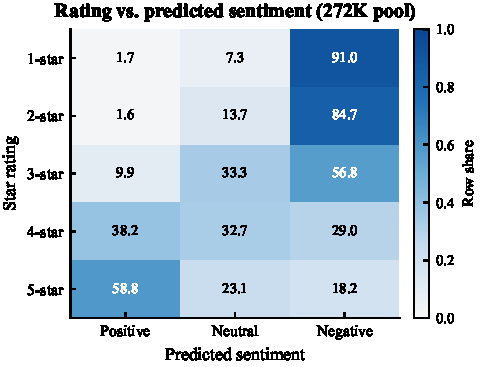
\includegraphics[width=0.62\textwidth]{fig_rating_crosstab.pdf}
\caption{Star rating versus predicted sentiment on the 272K confident
pseudo-label pool. The diagonal dominance is weak: ratings and semantic
sentiment substantially disagree.}
\label{fig:crosstab}
\end{figure}

\subsection{Stage-2 benchmark: lab2000}
\label{sec:lab2000-data}

To measure --- and then narrow --- the gold-to-corpus generalisation
gap documented in the lab500 pilot (Appendix~\ref{app:lab500}), we
constructed
\textbf{lab2000}: 2{,}000 corpus reviews in two disjoint, complementary
subsets.

\begin{itemize}
  \item \textbf{ood1000} (random OOD test): 1{,}000 reviews sampled
        uniformly at random from the 911K corpus (gold-deduplicated,
        cross-movie). This is a held-out evaluation set: no model in
        this paper trains on it.
  \item \textbf{al1000} (active-learning expansion): 1{,}000 reviews
        selected by margin/entropy sampling from the deployed student's
        predictions --- deliberately the hardest, most ambiguous rows
        (neutral-heavy, low-confidence). This is a \emph{training}
        set, not a test set.
\end{itemize}

\paragraph{Annotation protocol.} Each row was labelled independently
twice by two LLM annotation passes --- the \emph{same} annotator model
with different few-shot example sets, blind to star ratings and to
each other. This is single-model self-consistency, not two independent
annotators; Section~\ref{sec:iaa} discusses the implications for the
agreement numbers. Inter-pass agreement was 86.7\%
(Cohen's $\kappa = 0.80$) on ood1000 and 79.8\% ($\kappa = 0.67$) on
al1000 --- the lower agreement on al1000 is itself evidence that margin
sampling selects intrinsically ambiguous rows. All 335 inter-pass
disagreements plus 144 spot-checked agreements were adjudicated by the
author (479 human-adjudicated rows total: 200 in ood1000, 279 in
al1000); the remaining rows take the two-pass consensus label, so the
released labels are mixed-provenance (ood1000: 200 human + 800
consensus; al1000: 279 human + 721 consensus). Final distributions:
ood1000 = 398 positive / 327 neutral / 275 negative; al1000 = 473 /
369 / 158. A separate 200-row random subset of ood1000 was
blind-labelled by a second human annotator to measure agreement with
the released reference labels (Section~\ref{sec:iaa}).

%=====================================================================
\section{Methodology}
\label{sec:method}

\subsection{Overview}

The deployed system is a hybrid ensemble with three channels sharing a
common backbone pass where possible:

\begin{enumerate}
  \item \textbf{Distilled student}: MacBERT-base fine-tuned by
        distillation from a 7-channel teacher ensemble (Section~\ref{sec:distill}).
  \item \textbf{Frozen judge}: MegatronBERT-1.3B kept frozen; a small MLP
        head on its 4096-dimensional features (Section~\ref{sec:judge}).
  \item \textbf{Neutral specialist}: probability of neutrality computed
        from a corpus-trained detector blended with a judge-feature
        head (Section~\ref{sec:neu}).
\end{enumerate}

Figure~\ref{fig:arch} shows the data flow.

\begin{figure}[H]
\centering
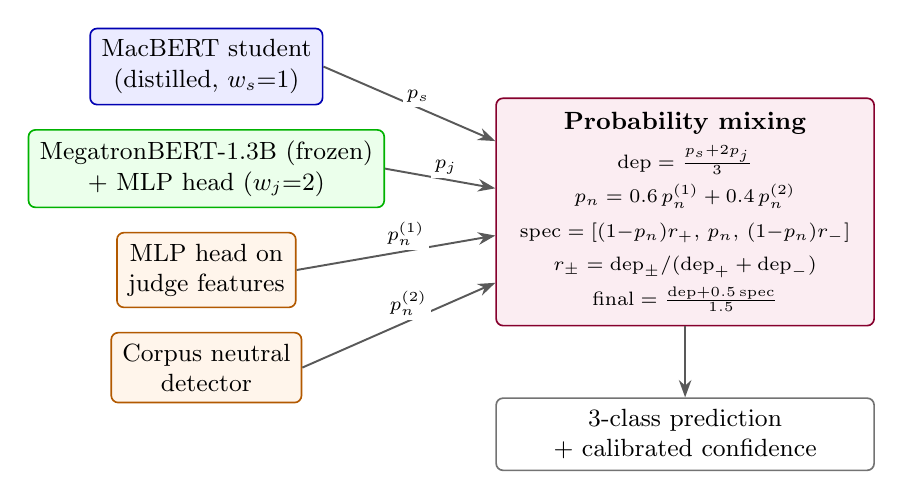
\begin{tikzpicture}[
  box/.style={draw=black!55,rounded corners=2.5pt,align=center,
              inner sep=4pt,font=\small,minimum height=8mm,
              fill=white,line width=0.6pt},
  ch/.style={box,fill=#1!8,draw=#1!70!black},
  arr/.style={-{Stealth[length=2.2mm,width=1.6mm]},line width=0.7pt,
              draw=black!65},
  lbl/.style={font=\scriptsize,fill=white,inner sep=1.5pt}]
\node[ch=blue]   (stu)  {MacBERT student\\(distilled, $w_s{=}1$)};
\node[ch=green, below=3mm of stu]   (judge) {MegatronBERT-1.3B (frozen)\\+ MLP head ($w_j{=}2$)};
\node[ch=orange,below=3mm of judge] (neu1)  {MLP head on\\judge features};
\node[ch=orange,below=3mm of neu1]  (neu2)  {Corpus neutral\\detector};
\node[box,fill=purple!7,draw=purple!70!black,anchor=west,
      minimum width=48mm,inner sep=5pt]
  (mix) at ([xshift=14mm,yshift=-5.5mm]judge.east) {%
  \textbf{Probability mixing}\\[3pt]
  {\scriptsize $\mathrm{dep}=\frac{p_s+2p_j}{3}$}\\[1.5pt]
  {\scriptsize $p_n=0.6\,p_n^{(1)}+0.4\,p_n^{(2)}$}\\[1.5pt]
  {\scriptsize $\mathrm{spec}=[(1{-}p_n)r_+,\,p_n,\,(1{-}p_n)r_-]$}\\[1pt]
  {\scriptsize $r_\pm=\mathrm{dep}_\pm/(\mathrm{dep}_++\mathrm{dep}_-)$}\\[1.5pt]
  {\scriptsize $\mathrm{final}=\frac{\mathrm{dep}+0.5\,\mathrm{spec}}{1.5}$}};
\node[box,below=9mm of mix,minimum width=48mm] (out) {3-class prediction\\+ calibrated confidence};
% four distinct entry points on the mix node's west edge (top to bottom)
\coordinate (in_s)  at ([yshift=9mm]mix.west);
\coordinate (in_j)  at ([yshift=3mm]mix.west);
\coordinate (in_n1) at ([yshift=-3mm]mix.west);
\coordinate (in_n2) at ([yshift=-9mm]mix.west);
\draw[arr] (stu.east)   -- node[lbl,above,pos=0.55] {$p_s$}       (in_s);
\draw[arr] (judge.east) -- node[lbl,above,pos=0.55] {$p_j$}       (in_j);
\draw[arr] (neu1.east)  -- node[lbl,above,pos=0.55] {$p_n^{(1)}$} (in_n1);
\draw[arr] (neu2.east)  -- node[lbl,above,pos=0.55] {$p_n^{(2)}$} (in_n2);
\draw[arr] (mix.south) -- (out.north);
\end{tikzpicture}
\caption{Deployed v3 architecture. $p_s,p_j,\mathrm{dep},\mathrm{spec},
\mathrm{final}\in\Delta^{3}$ are three-class probability vectors, whereas
$p_n^{(1)},p_n^{(2)},p_n\in[0,1]$ are scalar neutral probabilities;
$w_s,w_j$ are fusion weights, not model parameters. $r_\pm$ denote the
positive/negative shares of $\mathrm{dep}$ renormalised to sum to one.
The two MegatronBERT-based heads share one frozen-backbone feature
pass; the neutral specialist blends a judge-feature MLP with a
corpus-trained MacBERT detector.}
\label{fig:arch}
\end{figure}

\subsection{Teacher ensemble and distillation}
\label{sec:distill}

A 7-channel teacher ensemble --- TF-IDF logistic regression, frozen-
backbone MLP heads on MacBERT, MegatronBERT-1.3B and Erlangshen
variants, all trained on the 600 gold rows with honest out-of-fold
predictions --- reaches 86.8\% three-class accuracy. We distil it into
a single chinese-macbert-base student using hard-label
cross-entropy plus soft-target KL divergence
($\alpha=0.5$, temperature $\tau=2$, 8 epochs, 5-fold OOF). The student
alone reaches 80.2\%/74.2\%; blended 1:2 with the judge it reaches
87.8\%/81.8\%. Its role in the deployed system is to provide a cheap,
well-calibrated channel that also serves as the pseudo-labeller for
the corpus (Section~\ref{sec:flywheel}).

\subsection{Frozen judge}
\label{sec:judge}

\code{IDEA-CCNL/Erlangshen-}\hspace{0pt}\code{MegatronBert-1.3B-Sentiment} provides a
1.3B-parameter backbone pretrained with a sentiment-aware objective. We
keep it frozen and train a small MLP head on its 4096-d features over
the gold set. The deployed mixture weights the judge double the
student:
\[
  \mathrm{dep} = \tfrac{1}{3}\,p_{\text{student}} +
                \tfrac{2}{3}\,p_{\text{judge}} .
\]
The two MLP heads (binary and three-class) share a single backbone
feature pass via a cache, so the judge costs one forward pass per
request regardless of task.

\subsection{Pseudo-label flywheel}
\label{sec:flywheel}

The deployed student labels all 910{,}998 corpus reviews. The confident
subset ($\max p \ge 0.7$) contains 271{,}905 rows: 56.5K positive,
68.6K neutral, 146.8K negative. This pool is the raw material for every
corpus-scale model in Section~\ref{sec:corpus}. A second flywheel round
was tested and rejected: re-labelling with round-2 models produces
degenerate probabilities (mean confidence 0.986, memorisation), so
exactly one round is used. This saturation is consistent with the
confirmation-bias dynamics documented for self-training and pseudo-
labelling \citep{arazo2020,xie2020,sohn2020}: once the pseudo-labels
encode the teacher's own decision boundary, additional rounds amplify
self-consistency rather than add information.

\subsection{Neutral specialist}
\label{sec:neu}

The neutral class is the weakest link (92 gold examples). We attack it
on two fronts.

\paragraph{Corpus-trained detector.} A MacBERT binary classifier is
trained on a 115{,}000-row pseudo-labelled subset of the confident
pool, sampled with a per-class cap of 60K rows per side, teaching the
boundary between ``genuinely neutral'' and ``polarised'' reviews.

\paragraph{Specialist blend.} The probability of neutrality combines a
judge-feature MLP head and the corpus detector:
\[
  p_n = 0.6 \cdot P_{\text{neu}}(\text{MLP on judge feats})
      + 0.4 \cdot P_{\text{neu}}(\text{corpus detector}).
\]
From the dependency prediction $\mathrm{dep}=(d_+,d_n,d_-)$ we take the
positive/negative shares renormalised to sum to one,
$r_+ = d_+/(d_+ + d_-)$ and $r_- = d_-/(d_+ + d_-)$, replace the
neutral mass by the specialist estimate $p_n$, and form the
specialist distribution
\[
  \mathrm{spec} = \bigl[(1-p_n)\,r_{+},\; p_n,\;
                    (1-p_n)\,r_{-}\bigr],
\]
then blend it into the final output:
\[
  \mathrm{final} = \frac{\mathrm{dep} + 0.5\,\mathrm{spec}}{1.5}.
\]
Every weight ($0.6/0.4$ detector mix, $0.5$ blend) was selected by
20 random half-splits of the gold set and is stable across
$w \in [0.3, 0.6]$.

\subsection{Corpus-scale students}
\label{sec:corpus}

Using the 271{,}905-row pool, we trained corpus-only models (zero gold
training) to measure how far pseudo-labels alone can go: a balanced
160K-row three-class student, a 195K-row binary student, a 115K-row
neutral detector v1, and a hard-negative-mined v2 (rejected). These
models double as baselines and as candidates for ensemble channels;
Section~\ref{sec:results} reports which (if any) survived.

\subsection{Calibration}
\label{sec:calib}

The raw ensemble is strongly under-confident (ECE = 0.251: predictions
at 0.7--0.8 confidence are 98.9\% accurate). We fit a single temperature
$T = 0.37$ by NLL on the gold-600 OOF predictions, reducing ECE to
$\approx$0.04 without changing any predicted label or accuracy. $T$ is
applied at inference so displayed confidence is honest. Calibration
also transfers better after AL training: on ood1000 the scaled AL
mixes reach ECE $0.027$--$0.063$ vs.\ v3's 0.159 at $T{=}1$ ---
pseudo-labelled boundary data sharpens confidence, not just accuracy.

\subsection{Deployment}
\label{sec:deploy}

A FastAPI backend serves predictions; a React/Vite frontend provides the
demo UI. An exact-match lexicon guard intercepts ultra-short slang
before any GPU work. Warm latency is $\approx$0.1\,s per review on an
AMD RX 9070 GRE (ROCm); cold start $\approx$14\,s.

%=====================================================================
\section{Experimental Setup}
\label{sec:setup}

\paragraph{Evaluation protocol.} All headline numbers are
\textbf{stratified 5-fold out-of-fold} predictions on the 600-row gold
set: every model predicts only rows it never trained on. Corpus-scale
models are additionally evaluated on a 4{,}000-row \emph{silver} sample
of fresh corpus reviews scored against rating-implied labels.

\paragraph{Metrics.} Accuracy and macro-F1 (3-class), per-class
precision/recall/F1, neutral recall specifically, and ECE for
calibration. Significance is tested with McNemar's test on discordant
pairs and percentile bootstrap on $\Delta$F1; robustness is checked
with 20 random half-splits.

\paragraph{Baselines.}
\begin{itemize}
  \item TF-IDF (char $n$-gram) + logistic regression, gold-trained.
  \item StructBERT sentiment classifier (Ali DAMO), zero-shot binary;\\
        \footnotesize\code{damo/nlp\_structbert\_sentiment-classification\_chinese-base}
  \item Qwen3-0.6B / 1.7B / 4B chat models, zero-shot and 3-shot,
        scored by label log-probabilities.
\end{itemize}

%=====================================================================
\section{Results}
\label{sec:results}

\subsection{Main results}

\begin{table}[H]
\centering\small
\caption{Gold-600 results. ``Deployed'' rows are the production system
(5-fold out-of-fold); StructBERT and Qwen rows are zero-shot external
baselines --- StructBERT is binary-only and scored on the 508
non-neutral base rows. ``---'' = metric not reported.}
\label{tab:main}
\begin{tabular}{llcc}
\toprule
System & Task & Acc & Macro-F1 \\
\midrule
TF-IDF + LR            & 3-class & 0.7233 & 0.6188 \\
TF-IDF + LR            & binary  & 0.8406 & 0.8232 \\
StructBERT (DAMO)      & binary  & 0.8661 & 0.8459 \\
Qwen3-4B zero-shot     & 3-class & 0.7833 & 0.7348 \\
Qwen3-1.7B zero-shot   & 3-class & 0.7067 & 0.5739 \\
Qwen3-0.6B zero-shot   & 3-class & 0.6817 & 0.4764 \\
Teacher ensemble (7ch) & 3-class & 0.8680 & ---    \\
Deployed v2            & 3-class & 0.8900 & 0.8432 \\
\textbf{Deployed v3}   & \textbf{3-class} & \textbf{0.8950} & \textbf{0.8594} \\
Deployed v3            & binary  & 0.9587 & 0.9558 \\
\bottomrule
\end{tabular}
\end{table}

The deployed system beats the TF-IDF baseline by $+17.2$pp accuracy and
zero-shot Qwen3-4B by $+11.2$pp. (3-shot variants were also measured:
few-shot helps slightly at 4B --- 78.8\% vs.\ 78.3\% --- but collapses
at 1.7B, 51.0\%, due to negative-class bias; we report zero-shot as the
primary baseline.) Per-class metrics (3-class):
positive P/R/F1 = 0.909/0.943/0.926; neutral = 0.765/0.707/0.735;
negative = 0.931/0.906/0.918. Neutral recall improved 54.3\% $\to$
63.0\% (v2) $\to$ 70.7\% (v3) across expert iterations.
Figure~\ref{fig:confusion} shows the v3 confusion matrix: remaining
errors concentrate in neutral$\leftrightarrow$polar confusions
(47/63).

\begin{figure}[H]
\centering
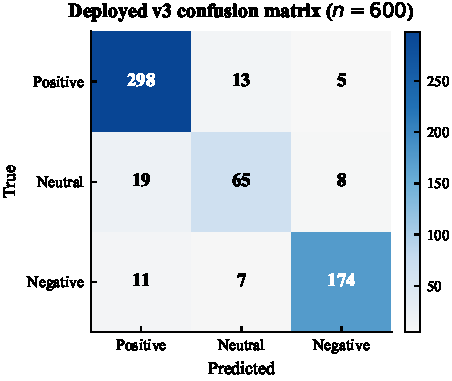
\includegraphics[width=0.55\textwidth]{fig_confusion.pdf}
\caption{Deployed v3 confusion matrix on the 600-row gold set
(out-of-fold). Row sums match the class distribution
(316/92/192).}
\label{fig:confusion}
\end{figure}

\subsection{Corpus-scale single models}

\begin{table}[H]
\centering\small
\caption{Corpus-trained models evaluated on gold-600 (zero gold
training unless noted). ``---'' = metric not reported.}
\label{tab:corpus}
\begin{tabular}{llccc}
\toprule
Model & Train data & Acc & Macro-F1 & Neu recall \\
\midrule
TF-IDF + star-rating labels & 300K rating  & 0.6183 & 0.5369 & ---    \\
TF-IDF + pseudo labels      & 200K pseudo  & 0.8117 & 0.7766 & ---    \\
MacBERT binary (rating)     & 115K rating  & 0.9232 & 0.9184 & ---    \\
MacBERT neutral v1          & 115K pseudo  & 0.9017 & 0.8328 & ---    \\
MacBERT binary pseudo       & 195K pseudo  & 0.9488 & 0.9455 & ---    \\
MacBERT 3-class pseudo      & 160K pseudo  & 0.8750 & 0.8463 & \textbf{0.848} \\
\bottomrule
\end{tabular}
\end{table}

The pseudo-label 3-class student alone reaches 87.5\%/84.6 with 84.8\%
neutral recall --- nearly matching the deployed ensemble. This is the
central empirical finding: \textbf{label quality at scale dominates
model capacity}. The same MacBERT architecture trained on star ratings
instead of pseudo-labels collapses on the three-class task.

\subsection{Pseudo-label scaling}

\begin{figure}[H]
\centering
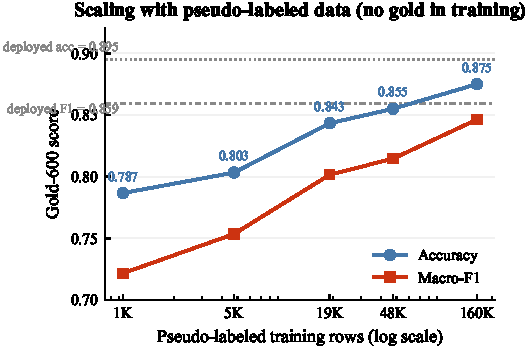
\includegraphics[width=0.68\textwidth]{fig_scaling.pdf}
\caption{Accuracy and macro-F1 of corpus-trained pseudo-label students
on gold-600 versus training-set size (log scale). \emph{Zero gold
training}: gold-600 is the held-out evaluation set only and is never
used for training. The dashed reference is the deployed ensemble
(accuracy 0.895, macro-F1 0.859). The y-axis starts at 0.70 to
highlight the performance differences. Performance grows monotonically
and is still rising at 160K rows.}
\label{fig:scaling}
\end{figure}

Table~\ref{tab:scaling} and Figure~\ref{fig:scaling} show a monotone
scaling curve: $\sim$1K rows $\to$ 78.8\%, 5K $\to$ 80.3\%, 19K $\to$
84.3\%, 48K $\to$ 85.5\%, 160K $\to$ 87.5\%. The curve has not saturated
--- corpus scale, not model size, is the active ingredient within the
ranges tested.

\begin{table}[H]
\centering\small
\caption{Pseudo-label scaling (gold-600 eval; no gold rows in training).
``---'' = metric not reported.}
\label{tab:scaling}
\begin{tabular}{lccc}
\toprule
Pseudo rows & Acc & Macro-F1 & Neutral recall \\
\midrule
$\sim$1K   & 0.7883 & 0.7237 & --- \\
$\sim$5K   & 0.8033 & 0.7535 & --- \\
$\sim$19K  & 0.8433 & 0.8016 & --- \\
$\sim$48K  & 0.8550 & 0.8146 & --- \\
$\sim$160K & 0.8750 & 0.8463 & 0.848 \\
\bottomrule
\end{tabular}
\end{table}

\subsection{Cross-domain silver evaluation}

On 4{,}000 fresh corpus reviews scored against rating-implied labels,
the round-3 student (trained on v3-teacher pseudo-labels) reaches 0.580
three-class / \textbf{0.837 binary} agreement versus rating, versus
0.552/0.803 for the round-1 student. Ensemble-derived labels transfer
slightly better out-of-domain even where gold scores are equal.

%=====================================================================
\section{Analysis}
\label{sec:analysis}

\subsection{Calibration}

\begin{figure}[H]
\centering
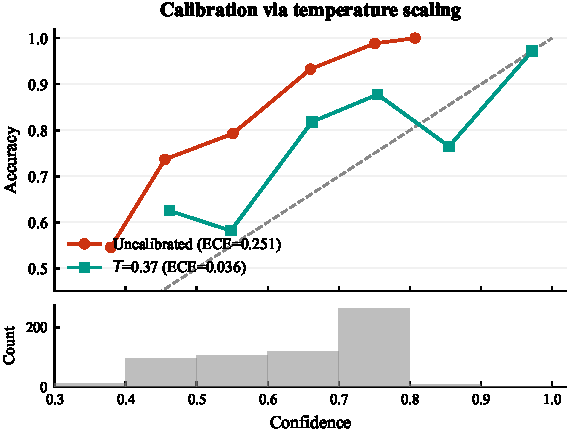
\includegraphics[width=0.85\textwidth]{fig_calibration.pdf}
\caption{Reliability diagram before and after temperature scaling
($T=0.37$, fitted by NLL on the gold-600 OOF predictions; all
quantities are computed on the same 600 out-of-fold rows). The lower
panel shows the sample count per equal-width confidence bin; the
high-confidence region is sparse, so local fluctuations are expected
even though the global ECE improves substantially. The accuracy axis
is truncated at 0.45 to show the pre-scaling miscalibration.}
\label{fig:calib}
\end{figure}

The raw ensemble is under-confident (ECE 0.251); temperature scaling
with $T=0.37$ reduces ECE to $\approx$0.04 (Figure~\ref{fig:calib})
without altering any predicted label or accuracy --- it only reshapes
the confidence distribution. One caveat: ECE averages over all bins,
so a handful of sparse bins can still deviate noticeably even though
the aggregate calibration improves substantially. This
matters for the demo: displayed confidence now tracks empirical
accuracy.

\subsection{Statistical significance}

v3 vs.\ v2: McNemar's test \citep{mcnemar1947} on discordant pairs
gives $p = 0.65$ (11 vs.\ 8); a paired bootstrap over resampled
evaluation rows \citep{efron1993} gives a 95\% CI on $\Delta$F1 of
$[-0.5, +3.9]$pp. Following standard practice for comparing
classifiers \citep{dietterich1998,demsar2006}, we treat differences
inside the CI as unresolved. The point estimate
($+1.6$pp F1, $+7.7$pp neutral recall) is consistent across 20 random
half-splits for every detector weight $w \in [0.3,0.6]$. We report this
honestly: the improvement is real but modest, and at $n=600$ the gold
set cannot resolve differences below $\sim$1pp.

\subsection{Error analysis}

Of the 63 errors that remain, 47 involve neutral$\leftrightarrow$polar
confusions, and most sit on reviews that even human annotators find
ambiguous --- mean confidence on errors is 0.51 versus 0.66 on
correct predictions. Reviews that state an explicit score
(``7.6/10'', ``三星半''; $n=56$) behave quite differently: only 5.4\%
of them are misclassified, compared with 11.0\% elsewhere. The model
clearly exploits overt rating cues when they are present; just 6 of
the 56 explicit scores even disagree with the semantic label.

\subsection{Rejected architectures}

More than twenty alternative designs were implemented, measured, and
rejected; the deployed v3 is the measured optimum. Among the documented
rejects: a neutral-gate cascade (its threshold overfit --- split-half
validation collapses from 87.6\% to 86\%), corpus-trained MLP heads as judge
replacement, student-probability averaging, self-distillation round 2,
stacked logistic meta-learner (0.837/0.794 --- channels too correlated
for 600 samples), class-weighted and max-len-128 students, Erlangshen
110M/330M students (pathologically slow on ROCm), neutral-detector v2
(worse in every ensemble combination), r3 self-training on v3-teacher
labels (student 0.8767/0.8434, all mixes below v3), gold-mixed corpus
training (circular gold evaluation --- flagged, not cited as a result),
Qwen3-4B synthetic augmentation (poisoned training: 79.2\%
standalone), and, in the Stage-2 OOD setting: AL-only training
(56.0\% --- margin sampling without a gold anchor collapses the class
prior) and gold+al soft-label distillation (71.0\% vs.\ 71.4\% for
hard-label SFT --- the narrow-domain teacher's OOD bias transfers
through soft targets).

\subsection{Comparison with a commercial training platform}

For completeness we compared against a commercial NLP training platform
(Alibaba Cloud PAI, StructBERT classifier, same 600-row task). Its
published page reported 89.83\% accuracy, but the per-class metrics on
the same page imply only 86.05\% accuracy / 83.23\% macro-F1 on an
effective validation set of \textbf{43 rows} (the three headline
numbers correspond to denominators 59/60/119 and cannot be
mutually reconstructed; the support-weighted recomputation also fails
to close). A Wilson interval on 43 rows spans [72.7\%, 93.4\%] --- the
sample size cannot distinguish 86\% from 90\%. Training-set self-
evaluation reached 99.02\% ($n=511$), a $\sim$13pp generalisation gap.
By contrast, our 89.5\%/85.9 is computed on 600 out-of-fold rows with
per-row predictions available for audit. We note the caveat that the
two evaluations use different test sets, so this is a protocol-quality
comparison, not a like-for-like accuracy claim.

%=====================================================================
\section{Stage-2: The lab2000 OOD and Active-Learning Study}
\label{sec:lab2000}

The lab500 pilot showed that gold-600 performance does not transfer to
terse corpus reviews and that LLM reference labels are too noisy to
serve as ground truth. We therefore built lab2000
(Section~\ref{sec:lab2000-data}) and ran a full
exposure-and-mitigation study. (The lab500 protocol and numbers are
retained in Appendix~\ref{app:lab500} for completeness.)

\subsection{Exposing the OOD gap}
\label{sec:ood-expose}

Table~\ref{tab:ood} reports every system on the held-out ood1000 set.
The deployed v3 --- trained exclusively on gold-600 --- drops from
89.5\% in-domain to \textbf{65.0\%} three-class accuracy (binary
pos/neg: 85.0\%). The gap is concentrated exactly where the lab500
pilot predicted: the neutral boundary.

\begin{table}[H]
\centering\small
\caption{ood1000 results. ``SFT'' = MacBERT fine-tuned on the listed
training data; ``mix'' = probability average of v3 and the SFT model,
with the fusion weight selected by stratified 5-fold cross-validation
on ood1000 --- each prediction uses weights tuned on the other folds,
so no reported row's label influences its own mix weight. Binary
evaluation excludes neutral examples. ``---'' = metric not reported
for this run. lab2000 labels are mixed-provenance: 479
human-adjudicated rows (200 ood + 279 al) plus two-pass LLM consensus
labels for the rest (Section~\ref{sec:lab2000-data}).}
\label{tab:ood}
\begin{tabular}{llcc}
\toprule
System & Training data & 3-class acc / F1 & Binary acc / F1 \\
\midrule
Deployed v3 (ensemble)      & gold-600        & 0.650 / 0.644 & 0.850 / 0.849 \\
SFT student                 & gold-600        & 0.626 / 0.611 & 0.832 / 0.831 \\
SFT student                 & al1000 only     & 0.560 / 0.519 & 0.577 / 0.512 \\
SFT student                 & gold-600+al1000 & 0.714 / 0.710 & 0.880 / 0.875 \\
SFT student (distilled)     & gold-600+al1000 & 0.710 / ---   & 0.825 / ---   \\
\textbf{mix (deployed cand.)}& gold-600+al1000 & \textbf{0.720 / 0.717} & \textbf{0.878 / 0.876} \\
\bottomrule
\end{tabular}
\end{table}

\begin{figure}[H]
\centering
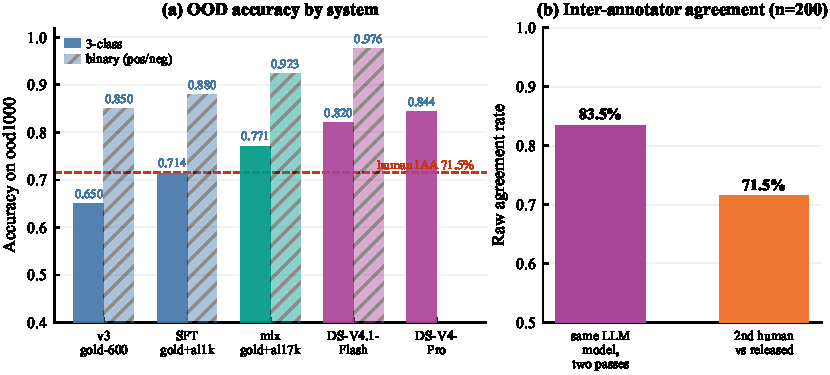
\includegraphics[width=0.95\textwidth]{fig_lab2000.pdf}
\caption{(a) ood1000 accuracy by system; the first three groups are
our local models and the last two are off-the-shelf DeepSeek LLMs
(the local Qwen3-4B baseline from Table~\ref{tab:llm} is omitted for
space); the dashed line marks the measured 71.5\% second-annotator
agreement with the released labels. (b) Raw pairwise agreement on the
same 200-row subset: two passes of the same LLM annotator model vs.\
a second human annotator scored against the released (mixed-provenance)
labels. Raw agreement rate is reported here, not Cohen's $\kappa$;
higher LLM self-agreement reflects shared inductive bias (same model)
and literal rubric following rather than superior annotation
quality.}
\label{fig:lab2000}
\end{figure}

Adding the 1{,}000 actively-selected AL rows (279 human-adjudicated +
721 LLM-consensus labels) to the
training set lifts three-class OOD accuracy by \textbf{+8.8pp}
(62.6\%$\to$71.4\%, McNemar $p = 4.0\times10^{-8}$) --- a gain that was
statistically unresolvable at $n{=}600$ ($p = 0.65$ for v3-vs-v2). The
ensemble mix reaches \textbf{72.0\% / 0.717} three-class and
\textbf{87.8\% / 0.876} binary under cross-fit weight selection ---
the improvement is not test-set overfitting by construction.

\subsection{Three empirical observations invisible at $n{=}600$}
\label{sec:findings}

\paragraph{F1: Active learning needs an anchor.} Training on al1000
\emph{alone} collapses to 56.0\% --- worse than gold-600 alone
(62.6\%). Margin sampling selects boundary cases and systematically
distorts the class prior; without the gold anchor the model loses its
reference for ordinary high-confidence reviews. Gold and AL are
complements, not substitutes.

\paragraph{F2: Under domain shift, hard labels may beat soft
distillation.} The gold+al teacher's soft targets transfer at 71.0\%
three-class vs.\ 71.4\% for hard-label SFT --- a 0.4pp gap that is
within noise at $n{=}600$, so we report it as directional only. The
direction is nonetheless consistent with the documented tendency of
teachers to transmit their own biases through soft probabilities under
distribution shift \citep{zhang2023shiftkd}.

\paragraph{F3: Ratings beat text exactly where text fails.} On the
al1000 ambiguity set, the star-rating rule reaches 64.3\% agreement
with the adjudicated labels while the text-only deployed model reaches
$\approx$47\%. When review text is maximally ambiguous --- the regime
margin sampling selects for --- the author's star rating is the only
remaining attitude signal. This closes the loop with
Section~\ref{sec:ratings}: ratings are a weak proxy on average, but a
strong disambiguator at the text-entropy ceiling. We flag this as an
exploratory observation on a small, disagreement-enriched subset, not
a general claim.

\subsection{Human agreement: the annotator-agreement reference}
\label{sec:iaa}

To bound what ``correct'' even means on wild short reviews, a 200-row
random subset of ood1000 was blind-labelled by a second human
annotator. Agreement with the released reference labels is
\textbf{71.5\%} (Cohen's $\kappa = 0.568$, bootstrap 95\% CI
$[0.47, 0.66]$) --- note this is a human-vs-reference agreement, not a
pure human--human figure: on this subset the reference labels are 47
human-adjudicated and 153 two-pass LLM-consensus rows. The
disagreement is not uniform: on items the first annotator labelled
neutral, the second agrees only 49\% of the time, relabelling 37 of 80
as positive. Two humans do not share a stable neutral boundary.
Model errors concentrate on exactly these ambiguous rows: the best AL
mix (al17k) scores 79.5\% on annotator-agreement items vs.\ 61.7\% on
disagreement items (v3: 67.8\% vs.\ 46.6\%), and AL training lifts
neutral recall on disagreement rows from 0.41 to 0.77
(Figure~\ref{fig:lab2000}).

Meanwhile our best OOD system scores \textbf{77.1\%} three-class after
AL scaling (72.0\% with al1000 labels alone) --- above the
measured 71.5\% second-annotator agreement reference, though the two
quantities are not strictly comparable (accuracy vs.\ pairwise
agreement, and the reference side is majority LLM-consensus). The
appropriate reading is not ``the model is imperfect'' but ``the model
has reached the human consistency range; residual error is dominated
by annotator-level ambiguity.'' For reference, the two LLM annotation
passes (same model, different few-shot prompts, blind to each other
and to star ratings) agree with each other at 83.5\% raw agreement
($\kappa = 0.75$) on the same subset --- higher than the 71.5\%
human reference, but this is single-model self-consistency inflated
by shared inductive bias and literal rubric following, not evidence of
superior annotation quality; which is why human adjudication, not LLM
consensus, anchors the final labels.

\subsection{Comparison with a frontier LLM}
\label{sec:llm}

A natural reviewer question is whether a large general-purpose LLM
obviates the whole pipeline. We evaluated DeepSeek-V4.1-Flash (a
$\sim$763B-parameter API model) and DeepSeek-V4-Pro ($\sim$1.6T
parameters) zero-shot on the
same adjudicated labels, with a compact JSON-only prompt and
low reasoning effort.

\begin{table}[H]
\centering\small
\caption{Frontier-LLM vs.\ local pipeline on lab2000 (API snapshots
evaluated November 2026). Parse failures
are excluded from accuracy denominators and reported separately.
Latency is mean per-request wall time. ``---'' = metric not reported.}
\label{tab:llm}
\begin{tabular}{lcccc}
\toprule
System & Params & ood1000 3-class & ood1000 binary & Latency \\
\midrule
DeepSeek-V4-Pro     & $\sim$1.6T     & 0.844 (n=950) & --- & $\sim$5.9s API \\
DeepSeek-V4.1-Flash & $\sim$763B    & 0.820 (n=992) & \textbf{0.976} (n=661) & $\sim$1.7s API \\
Qwen3-4B (local)    & $\sim$4B      & 0.706 (n=1000) & --- & $\sim$2.3s local \\
Deployed v3         & $\sim$1.5B    & 0.650 & 0.850 & $\sim$0.1s local \\
SFT+mix (gold+al17k) & $\sim$1.6B    & \textbf{0.771} & 0.923 & $\sim$0.1s local \\
\bottomrule
\end{tabular}
\end{table}

On the full random OOD set DeepSeek-V4.1-Flash leads by $\sim$5pp
(V4-Pro by $\sim$8pp) --- unsurprising given the orders-of-magnitude
parameter gap ($\sim$763B--1.6T vs.\ our 0.1--1.6B local models) and
the corpus exposure our student lacks (on the 992
jointly parseable rows vs.\ Flash, McNemar $p = 5.8\times10^{-4}$). Three
qualifications keep the comparison
honest. First, the neutral-class wall hits everyone: DeepSeek's own
binary accuracy (97.6\%) exceeds its three-class accuracy (82.0\%) by
15.6pp, the same polarity-vs-neutral gap we document --- intrinsic
ambiguity is not a small-model artefact. Second, on the human-adjudicated
hard subset (195 ood rows jointly parseable by DeepSeek) the gap
nearly closes: DeepSeek reaches
59.5\% on the ood portion vs.\ 59.0\% for our al1000
ensemble mix
(parity within noise); the subset is enriched for exactly the cases
where rubric-following and world knowledge diverge. Third, the
deployment economics differ by orders of magnitude: the local system
runs offline on a single consumer GPU at $\sim$0.1s/review with zero
per-token cost and no data leaving the machine, while the API model
requires network access, per-call billing, and ships user text to a
third party --- decisive constraints in privacy-sensitive deployments.
We therefore position the contribution not as ``beats LLMs'' but as
``task-calibrated compact model at the human-consistency range, at
edge-deployable cost.''

\subsection{Can LLM pseudo-labels replace human adjudication?}
\label{sec:ds-teacher}

The frontier-LLM result above suggests an obvious scaling path: if the
763B Flash model labels the AL set well, its labels may substitute for
expensive human adjudication. We tested this directly --- a MacBERT
student SFT'd on gold-600 + al1000 with \emph{DeepSeek-V4.1-Flash}
labels (987 parseable rows) instead of the released al1000 labels.

\begin{table}[H]
\centering\small
\caption{Released al1000 labels vs.\ DeepSeek pseudo-labels for AL
expansion (ood1000, mixed-provenance reference: 200 human +
800 LLM-consensus rows).}
\label{tab:ds-teacher}
\begin{tabular}{lcc}
\toprule
AL labels & 3-class acc / F1 & Binary acc / F1 \\
\midrule
gold-600 only              & 0.626 / 0.611 & 0.832 / 0.831 \\
gold-600 + al1000 (released)  & 0.714 / 0.710 & \textbf{0.880 / 0.875} \\
gold-600 + al1000 (DS-flash) & \textbf{0.713 / 0.714} & 0.863 / 0.860 \\
\bottomrule
\end{tabular}
\end{table}

DeepSeek pseudo-labels match the released labels on the three-class
task (71.3\% vs.\ 71.4\%) and trail slightly on binary (86.3\% vs.\
88.0\%). An ensemble mix at $0.5{:}0.5$ reaches 73.4\% (split-half
$0.734 \pm 0.015$), nominally above the al1000-label mix.

\paragraph{Scaling: 1K AL $\to$ 5.9K hybrid.} The parity result
raises the obvious question --- if LLM labels substitute for the
released al1000 labels at 1K, do they \emph{scale} where human
annotation cannot? We
sampled \textbf{al5000}: the next 5{,}000 margin/entropy-selected
corpus rows (same band and class quotas as al1000, disjoint from all
lab2000 texts), labelled them with DeepSeek-V4.1-Flash (4{,}906
parseable; label distribution 1{,}563 pos / 2{,}552 neu / 791 neg ---
neutral-heavy as designed), and trained the same SFT recipe. With
$\sim$6.5K AL rows the epoch optimum shifts to 4 (8 epochs overfits;
the e4-vs-e8 choice was made on ood1000, a single discrete
disclosure-level hyperparameter decision --- see
Section~\ref{sec:limits}).

\begin{table}[H]
\centering\footnotesize
\caption{AL-scaling on ood1000 (mixed-provenance labels: 479
human-adjudicated + two-pass LLM consensus; per-set split in
Section~\ref{sec:lab2000-data}). All rows are
gold-600 + listed AL data, MacBERT SFT. ``mix'' rows are probability
averages of v3 and the SFT model; the fusion weight is selected by
stratified 5-fold cross-validation (out-of-fold predictions, no row's
label influences its own weight). Ranges denote spread across random
seeds (five for three-class, four for binary).
Binary evaluation excludes neutral examples; ``---'' = not reported.}
\label{tab:al-scaling}
\begin{tabular}{lcc}
\toprule
AL training data & 3-class acc / F1 & Binary acc / F1 \\
\midrule
gold-600 only                        & 0.626 / 0.611 & 0.832 / 0.831 \\
gold-600 + al1000 (released)         & 0.714 / 0.710 & 0.880 / 0.875 \\
gold-600 + al1000 (DS labels)        & 0.713 / 0.714 & 0.863 / 0.860 \\
gold-600 + al5000 (DS labels)        & 0.719 / 0.720 & 0.893 / 0.890 \\
gold-600 + al6k (all DS labels)      & 0.725 / 0.727 & 0.893 / 0.890 \\
\textbf{gold-600 + al6k (hybrid)}    & \textbf{0.729 / 0.731} & \textbf{0.911 / 0.908} \\
gold-600 + al11k (1K AL + 9.9K DS)& 0.734 / 0.737 & \textbf{0.914 / 0.912} \\
gold-600 + al11k (1K AL + 4.9K DS + 5K Qwen3-4B) & 0.703 / 0.706 & 0.902 / 0.898 \\
gold-600 + al11k (all DS, no AL core) & 0.727 / 0.732 & 0.900 / 0.898 \\
gold-600 + al3k (disagreement-mined DS) & 0.703 / 0.704 & 0.877 / 0.874 \\
gold-600 + al14k (1K AL + 12.9K DS) & 0.744 / 0.747 & 0.914 / 0.911 \\
gold-600 + al17k (1K AL + 15.9K DS) & 0.730--0.746 / 0.732--0.749 & 0.915--0.924 / 0.912--0.922 \\
\midrule
+ v3 mix (al6kh)                     & 0.742 / 0.743 & 0.909 / 0.907 \\
+ v3 mix (al11kds, best of 3 seeds)    & 0.757 / 0.760 & --- \\
+ v3 mix (al11kds 3-seed avg)           & 0.749 / 0.752 & --- \\
+ v3 mix (al11kds binary e8)            & --- & 0.915 / 0.913 \\
+ v3 mix (al14kds, 3 seeds)          & 0.748--0.757 & --- \\
+ v3 mix (al14kds 3-seed avg)        & 0.755 / 0.758 & --- \\
+ v3 mix (al14kds binary)            & --- & 0.909 / 0.907 \\
+ v3 mix (al17kds, 5 seeds)          & 0.746--0.763 & --- \\
+ v3 mix (al17kds 5-seed avg)        & \textbf{0.771 / 0.774} & --- \\
+ v3 mix (al17kds binary e8 4-seed avg) & --- & 0.923 / 0.920 \\
\bottomrule
\end{tabular}
\end{table}

Two observations. First, \textbf{scale beats provenance}: 5{,}893
pure-LLM labels (72.5\%) already exceed the 1{,}000-row al1000 set's
mixed-provenance labels (71.4\%). The teachers' biases differ usefully: DeepSeek
under-calls \emph{positive} on ambiguous rows (only 65\% agreement
with released-label positives, relabelling 156/464 as neutral) while agreeing
with the released al1000 labels on neutral at 88\% --- the
human-adjudicated core corrects exactly
this polarity bias, which is why the hybrid wins. Second, the \textbf{hybrid is best}: keeping the al1000 set's
mixed-provenance labels on the hardest 1{,}000 rows and adding 4{,}906 LLM
labels reaches 72.9\% standalone and \textbf{74.2\% / 0.743} three-class
and \textbf{90.9\% / 0.907} binary after mixing --- the strongest OOD
numbers at this scale, still $\sim$7pp below the frontier LLM but at
$\sim$0.1s local latency.

\paragraph{Diminishing returns and teacher quality at scale.} We pushed
the same protocol to $\sim$11K AL rows twice: once adding a second
5{,}000 DeepSeek-labelled batch (al11k-DS), once replacing it with
5{,}000 labels from a \emph{local} Qwen3-4B teacher scored by
label-logprob (al11k-Qwen; the local model reaches only 70.6\% on
ood1000 zero-shot vs.\ DeepSeek's 82.0\%). The all-API-teacher run
edges the hybrid forward (73.4\% standalone, 91.5\% binary, and the
best gold-600 cross-fit of the 11K-scale models at 81.0\%), but the
three-class mix is statistically flat vs.\ 6K (74.9\% seed-averaged
vs.\ 74.2\%, McNemar $p = 0.56$) --- the
1K$\to$6K gain does not repeat at 6K$\to$11K, marking the
onset of diminishing returns in the ambiguity region. The gain over
the 1K-AL mix is nonetheless significant (McNemar $p = 0.041$,
109 vs.\ 80 discordant pairs), and the mix's OOD calibration improves
with it (ECE 0.037 vs.\ v3's 0.159). The local-teacher run is
clearly worse (70.3\% standalone, 72.4\% mixed, 90.2\% standalone
binary, cross-fit 79.5\%; pairwise McNemar vs.\ the DS-teacher mix reaches
$p = 0.041$ --- teacher quality is a real, measurable gap, not noise):
at identical scale, pseudo-label quality --- not
quantity --- is the binding constraint, and a 4B open teacher cannot
substitute for the frontier API here. The teachers' disagreement is
structured, not random: on the same 5{,}000 uncertainty-sampled rows
their labels agree on only 62.3\%, with Qwen over-calling positive
(725 of DeepSeek's neutral rows) and under-calling negative (396 of
its negative rows relabelled neutral) --- a distributional bias the
student faithfully inherits. An additional ablation replaces the
released al1000 labels with DeepSeek labels at the same 11K scale
(al11k-allDS): the three-class mix is unchanged (75.2\%,
McNemar $p = 0.81$ vs.\ the al1000 mix) while binary
drops $\sim$2.4pp to 89.2\% (McNemar $p = 0.014$) --- at this scale
the human-verification core's
marginal value concentrates in the polarity boundary, not the neutral
one. A third round then tests whether \emph{where} AL rows are drawn
matters at the margin: we mined 3{,}000 new rows from the
student-disagreement pool (rows where two independently-trained
student variants disagree on the argmax label), labelled them with
DeepSeek (al3kds), and added them
to form al14kds (1K AL + 12.9K DS). The 3K subset alone is
strikingly label-efficient --- 70.3\% standalone, 71.5\% mixed,
roughly matching the 1K-AL-label mix (72.0\%) at 3$\times$
the label count but API-token rather than adjudication cost --- while
the full 14K mix reaches \textbf{75.5\%} three-class
(74.8--75.7\% across three seeds, 75.5\% seed-averaged)
and \textbf{90.9\%} binary, with
gold-600 cross-fit 81.5\%. The difference over the best 11K seed is
within noise at
$n{=}1000$ (McNemar $p = 0.91$), and the 14K mix remains significantly
above the 1K-AL mix ($p \approx 0.01$, 107 vs.\ 72 discordant). A
fourth identical round (al17kds, another 3{,}000 disagreement-mined
DeepSeek rows) reaches \textbf{77.1\%} three-class seed-averaged
(74.6--76.3\% across five seeds) and
\textbf{92.3\%} binary, with gold-600 cross-fit 81.0\% --- the best
observed numbers, though +1.6pp over 14K is again within noise
(McNemar $p = 0.064$), confirming saturation in the $\sim$75--77\% band ---
the
honest reading is that disagreement-targeted sampling helps, but the
three-class curve is approaching its ceiling. The honest scaling curve is
therefore: rapid gains to $\sim$6K AL rows, then saturation on the
three-class task while binary and in-domain robustness keep improving.
The total API cost for all 15{,}906 additional DeepSeek labels was a
few hundred thousand tokens --- orders of magnitude cheaper than
equivalent human annotation.

\textbf{Stratification checks.} Two cuts address the obvious
objections. \emph{Provenance}: the al17k gain is not an artifact of
LLM-consensus labels --- on the 800 consensus rows the mix improves
over v3 by +12.7pp (69.6\%$\to$82.4\%) and on the 200
human-adjudicated rows by +9.5pp (46.5\%$\to$56.0\%). The
adjudicated subset is intrinsically harder (author adjudication
concentrated on inter-pass disagreements), yet the gain replicates
there. \emph{Length}: gains concentrate on terse reviews --- of the
+121 net discordant wins over v3, 58 fall on $\le$20-character rows
--- while the $>$100-character slice remains weakest for every system
(mix 72.4\% vs.\ v3 61.2\% on ood1000; 66.7\% on fresh500), consistent
with the length-as-domain-signal caveat in the router analysis below.
Calibration also improves with scale: OOD ECE falls from v3's 0.159
to 0.063 (al17k) and 0.027 (al14k).

\textbf{Fresh-sample robustness check.} Because AL rows were sampled
on corpus uncertainty and mix weights by cross-validation on ood1000,
we additionally sampled
\textbf{fresh500} --- 500 uniformly-random corpus reviews disjoint
from all training and eval texts (zero text overlap verified against
gold-600 and every AL pool through al17k) --- labelled by the same
DeepSeek teacher. With weights frozen at the ood1000 cross-fit values
($w_{\mathrm{SFT}}{=}0.6$ three-class, the modal fold weight; $0.5$
binary, the fold median --- the e8 binary fold weights are bimodal,
0.45--0.95), the headline al17kds mix scores \textbf{77.0\%}
three-class vs.\ v3's 58.8\% (McNemar $p = 9.1\times10^{-15}$) and
\textbf{93.7\%} binary vs.\ 86.3\% ($p = 1.9\times10^{-4}$) --- the AL
gain replicates on unseen data and is not an artifact of
benchmark-specific tuning. (The earlier al14k checkpoint scored
74.6\% / 92.6\% under the same protocol; the standalone al17k SFT
student reaches 78.0\% five-seed-averaged three-class on fresh500
--- the frozen ood1000-tuned mix weights do not transfer perfectly
to a new distribution.) (Caveat: fresh500 labels are
teacher-generated, not human gold, so these numbers measure
generalisation to the teacher's label distribution; binary, being
less ambiguous, is less affected by this alignment.)

The practical protocol this validates is exactly the one lab2000
itself used: \emph{LLM-label at scale, human-adjudicate a verification
core}. Future work (ii) of Section~\ref{sec:conclusion} is thereby
partially realised.

\paragraph{Deployment trade-off (measured, not assumed).} A natural
question is whether the OOD-hardened mix should replace v3 in the
demo. We tested this honestly: the SFT component was cross-fit on
gold-600 (5 folds, each holding out 120 gold rows while training on
the rest + all al1000), then mixed with v3's OOF probabilities. The
SFT student alone reaches only \textbf{80.0\% / 0.730} on gold-600
(80.2\% / 0.737 for the scaled al6k-hybrid variant, 81.0\% / 0.751 for
al11k-DS, 81.5\% for al14k-DS, 81.0\% for al17k-DS; vs.\ v3's 89.5\% /
0.859), and SFT-heavy mixture weights land at
80--82\% (lighter weights reach 85.8--88.5\%; no weight exceeds v3's
89.5\%) --- training on terse ambiguous AL examples shifts the
decision boundary away from the longer, single-film gold
distribution. OOD-hardening and in-domain accuracy are therefore in
tension here; we retain v3 as the deployed model and report the mix as
an OOD-specialist candidate. A length-aware router (short reviews
$\to$ mix, long $\to$ v3) traces a Pareto frontier rather than a free
lunch: at threshold 20 chars it gives 87.3\% gold / 71.0\% OOD,
between v3 (89.5\% / 65.0\%) and the pure mix ($\sim$82\% / 77.1\%).
Length is an imperfect domain signal (32\% of gold reviews are $<$50
chars; 26\% of ood1000 are $\ge$50), so we leave a learned
 domain router to future work. Table~\ref{tab:router} traces the
full frontier under a fixed fusion weight ($w_{\mathrm{SFT}}{=}0.6$,
the modal cross-fit value): every threshold buys OOD accuracy with
gold accuracy, with no dominant point.

\begin{table}[H]
\centering\footnotesize
\caption{Length-router frontier: reviews $\le T$ chars routed to the
AL mix, longer ones to v3 (fixed $w_{\mathrm{SFT}}{=}0.6$ fusion).
Gold-600 and ood1000 three-class accuracy; the pure-mix endpoint's
cross-fit OOF estimate is 0.771 (Table~\ref{tab:al-scaling}).}
\label{tab:router}
\begin{tabular}{lcc}
\toprule
Threshold $T$ & Gold-600 & ood1000 \\
\midrule
0 (pure v3)      & 0.895 & 0.650 \\
20               & 0.873 & 0.710 \\
50               & 0.865 & 0.742 \\
100              & 0.845 & 0.760 \\
$\infty$ (pure mix) & 0.822 & 0.774 \\
\bottomrule
\end{tabular}
\end{table}

\subsection{What lab2000 does not claim}
\label{sec:lab2000-caveats}

al1000 is a training set; its headline numbers (e.g.\ the rating-rule
comparison) characterise difficulty, not generalisation. The
human-adjudicated 479 rows are a non-random, disagreement-enriched
subset; accuracies on it are lower for every system and are reported
for the LLM comparison only. LLM-assisted pre-annotations were
adjudicated by a single human author plus a 200-row second-human
sample; the released data marks per-row provenance
(\code{final\_source}) so downstream users can restrict to the
479-row human-verified core if desired.

%=====================================================================
\section{Limitations and Threats to Validity}
\label{sec:limits}

\begin{itemize}
  \item \textbf{Domain narrowness (mitigated, not eliminated).} The
        gold set is 600 reviews from a \emph{single film page}; the
        lab2000 study quantifies the resulting OOD gap (65.0\%
        three-class) and shows 1{,}000 actively-selected rows
        (mixed-provenance labels) recover most of it (72.0\%), but ood1000 remains the only
        true held-out cross-movie test.
  \item \textbf{lab2000 label provenance.} Pre-annotations are
        LLM-generated; 479/2{,}000 rows carry human adjudication and a
        200-row second-human IAA sample ($\kappa = 0.57$). Consensus
        labels are reliable but not infallible; per-row
        \code{final\_source} is released.
  \item \textbf{Pseudo-label ceiling.} Pseudo labels inherit teacher
        biases; the flywheel saturates after one round (round-2 mean
        confidence 0.986 = memorisation). The lab2000 results suggest
        the teacher's narrow-domain prior is the binding constraint on
        OOD pseudo-labels.
  \item \textbf{Test-set-informed discrete choices.} Fusion weights
        are cross-fit, but two single discrete decisions were made
        using ood1000 feedback: the e4-vs-e8 epoch choice at scale
        (Section~\ref{sec:ds-teacher}) and per-task binary mix weights.
        These are disclosed rather than hidden, but a fully
        label-free protocol would avoid them.
  \item \textbf{Statistical power.} At $n=600$, differences below
        $\sim$1pp are unresolvable; the lab2000 OOD study ($n=1{,}000$)
        restores power for the headline Stage-2 claims, while
        gold-set micro-differences remain unresolved.
  \item \textbf{Engineering constraints.} The ROCm/Windows GPU stack
        required a driver-level reboot during 1.3B feature extraction;
        inference latency figures are single-GPU measurements.
\end{itemize}

%=====================================================================
\section{Conclusion and Future Work}
\label{sec:conclusion}

On a realistic low-resource Chinese sentiment task, corpus-scale
pseudo-labelling is the highest-leverage ingredient: it lifts neutral
recall from 54\% to 71\% and lets a single compact student nearly match
a multi-model ensemble. Specialist decomposition on corpus-trained
neutral detectors adds a further validated gain. Star ratings alone are
insufficient supervision --- measured, not assumed.

The lab2000 study then stress-tests the result honestly. The
gold-trained system drops to 65.0\% three-class on wild cross-movie
reviews; 1{,}000 actively-selected boundary examples
(279 human-adjudicated + 721 LLM-consensus labels)
recover the gap to 72.0\% (the underlying SFT gain: $+8.8$pp,
McNemar $p = 4.0\times10^{-8}$), and scaling the
same protocol with frontier-LLM pseudo-labels reaches \textbf{77.1\%}
three-class --- above the measured 71.5\% second-annotator agreement
reference --- and \textbf{92.3\%} binary.
Three empirical observations emerge: active learning requires a gold
anchor, hard labels may outperform soft distillation once the evaluation
domain shifts, and star ratings become the strongest available signal
precisely where review text is most ambiguous. Against frontier LLMs
of $\sim$763B--1.6T parameters the compact pipeline trails on raw OOD
accuracy but
reaches parity on human-adjudicated hard items at one-to-two
orders of magnitude lower latency and cost, with no data egress.

Future work: (i) scale the adjudicated AL set (the DS-teacher pilot in
Section~\ref{sec:ds-teacher} tests whether frontier-LLM pseudo-labels
can substitute for human adjudication at scale); (ii) use stronger LLM
teachers for corpus re-labelling to inject the world knowledge the
student lacks --- lab2000 shows this is the dominant residual gap;
(iii) test MacBERT-large students and the full 271K unbalanced pool;
(iv) domain-adversarial or multi-domain training to close the
gold$\to$corpus gap without per-domain annotation.

%=====================================================================
\section*{Reproducibility}
\addcontentsline{toc}{section}{Reproducibility}

\begin{sloppypar}
All scripts, out-of-fold predictions, experiment records, and the
lab2000 benchmark data are in the
project repository (\url{https://github.com/shuakami/douban-sentiment}).
The 910K corpus is external (research use only, not redistributed);
trained checkpoints are published at
\url{https://huggingface.co/Shuakami/douban-sentiment-weights}. The
full preprocessing $\to$ pseudo-label $\to$ train $\to$ evaluate
pipeline is scripted end-to-end.
Key artifacts: \code{out/ens\_lite\_3class\_v3.json} (deployed OOF
predictions + probabilities), \code{out/lab500\_*} (OOD study),
\code{data/lab2000/} (benchmark + teacher labels),
\code{scripts/} (all training/eval code), \code{PAPER.md} (condensed
report). Hardware: AMD RX 9070 GRE, ROCm, PyTorch bf16.
\end{sloppypar}

%=====================================================================
\appendix
\section{Training Details and Reproducibility}
\label{app:repro}

\subsection{Hyperparameters}

\begin{table}[H]
\centering\small
\caption{Key hyperparameters of the deployed pipeline.}
\label{tab:hparams}
\begin{tabular}{lll}
\toprule
Component & Setting & Value \\
\midrule
Distilled student & backbone & \code{hfl/chinese-macbert-base} \\
                   & distill $\alpha/\tau$ & 0.5 / 2 \\
                   & epochs / max-len & 8 / 256 \\
                   & folds (OOF) & 5 \\
Judge head         & backbone & MegatronBERT-1.3B (frozen) \\
                   & features & 4096-d (CLS + mean-pooled) \\
                   & head & 2-layer MLP \\
Neutral detector   & backbone & MacBERT-base \\
                   & train rows & 115{,}000 (per-class cap 60K, 2 epochs) \\
Pseudo pool        & confidence & $\max p \ge 0.7$ \\
                   & rows & 271{,}905 (56.5K/68.6K/146.8K) \\
Calibration        & method & temperature scaling \\
                   & $T$ & 0.37 (NLL on gold) \\
Ensemble weights   & dep & student 1 : judge 2 \\
                   & spec blend & 0.5 \\
                   & $p_n$ mix & 0.6 judge-head : 0.4 corpus detector \\
\bottomrule
\end{tabular}
\end{table}

\subsection{Artifacts}

\begin{itemize}
  \item \code{out/ens\_lite\_3class\_v3.json} --- deployed 3-class OOF
        predictions and probabilities (all 600 rows).
  \item \code{out/ens\_lite\_binary.json} --- deployed binary OOF.
  \item \code{out/lab500\_*} --- lab500 pilot: samples, two-pass LLM labels,
        predictions, cross-validation results.
  \item \code{data/reviews\_gold\_al1000.jsonl} + \code{data/lab2000/}
        --- lab2000 benchmark: 2{,}000 adjudicated labels with
        per-row provenance, dual-pass pre-annotations, DeepSeek/Qwen
        teacher predictions and labels, fresh500, and all Stage-2
        experiment outputs (see \code{data/lab2000/README.md}).
  \item \code{scripts/} --- end-to-end pipeline covering corpus
        preprocessing, pseudo-labelling, corpus-head training,
        distillation, and ensemble evaluation (full script list in the
        repository).
  \item \code{web/} + \code{web-ui/} --- FastAPI backend and React demo.
\end{itemize}

\subsection{Environment}

Python 3.12, PyTorch (ROCm), \code{transformers}, AMD RX 9070 GRE GPU.
All GPU jobs serialized (concurrent jobs crash the ROCm/Windows stack).
Model weights: MacBERT students $\sim$400MB each; MegatronBERT-1.3B
shared backbone; total deployed footprint under 4GB. Cold start
$\approx$14s, warm inference $\approx$0.1s per review.

%=====================================================================
\section{Appendix: The lab500 Pilot Study}
\label{app:lab500}

Before lab2000, a 500-row pilot measured the same OOD question with
weaker instrumentation. 500 reviews were sampled uniformly at random
from the 911K corpus (gold-deduplicated) and labelled independently by
two LLM annotators (a general-purpose assistant model and Qwen3-4B
zero-shot \citep{qwen2025}); the deployed v3 pipeline scored all rows.

\begin{table}[H]
\centering\small
\caption{lab500 pilot results (superseded by lab2000).
``---'' = metric not reported.}
\label{tab:lab500-app}
\begin{tabular}{llcc}
\toprule
Evaluator & Reference & $n$ & Accuracy \\
\midrule
v3 ensemble      & LLM-A labels      & 500 & 0.604 \\
Qwen3-4B         & LLM-A labels      & 500 & 0.662 \\
v3 ensemble      & two-pass LLM consensus & 331 & 0.740 \\
v3 binary        & LLM-A labels      & 255 & \textbf{0.918} \\
MacBERT CV       & held-out labels    & --- & 0.600 OOF \\
\bottomrule
\end{tabular}
\end{table}

Inter-annotator agreement between the two LLMs was only 66.2\%, and a
model trained on 400 in-domain labels reproduced held-out labels at
just 60\% OOF --- motivating the larger adjudicated lab2000 benchmark.
Rows the teacher found easy (confidence $\ge 0.7$) scored 0.757 for
every annotator pair; hard rows scored $\approx$0.53.

%=====================================================================
\begin{thebibliography}{99}\small

\bibitem[Devlin et al.(2019)]{devlin2019}
J.~Devlin, M.-W.~Chang, K.~Lee, K.~Toutanova.
\newblock \emph{BERT: Pre-training of Deep Bidirectional Transformers for Language Understanding}.
\newblock In \emph{Proceedings of NAACL-HLT}, pages 4171--4186, 2019.
\newblock \url{https://arxiv.org/abs/1810.04805}.

\bibitem[Liu et al.(2019)]{liu2019}
Y.~Liu, M.~Ott, N.~Goyal, J.~Du, M.~Joshi, D.~Chen, O.~Levy, M.~Lewis,
L.~Zettlemoyer, V.~Stoyanov.
\newblock \emph{RoBERTa: A Robustly Optimized BERT Pretraining Approach}.
\newblock \emph{arXiv preprint arXiv:1907.11692}, 2019.
\newblock \url{https://arxiv.org/abs/1907.11692}.

\bibitem[Cui et al.(2020)]{cui2020}
Y.~Cui, W.~Che, T.~Liu, B.~Qin, Z.~Yang, S.~Wang, G.~Hu.
\newblock \emph{Revisiting Pre-Trained Models for Chinese Natural Language Processing}.
\newblock In \emph{Findings of EMNLP}, pages 657--668, 2020.
\newblock \url{https://arxiv.org/abs/2004.13922}.

\bibitem[Wang et al.(2020)]{wang2020}
W.~Wang, B.~Bi, M.~Yan, C.~Wu, Z.~Bao, J.~Xia, L.~Peng, L.~Si.
\newblock \emph{StructBERT: Incorporating Language Structures into Pre-training for Deep Language Understanding}.
\newblock In \emph{International Conference on Learning Representations (ICLR)}, 2020.
\newblock \url{https://arxiv.org/abs/1908.04577}.

\bibitem[Sun et al.(2019)]{sun2019}
Y.~Sun, S.~Wang, Y.~Li, S.~Feng, X.~Chen, H.~Zhang, X.~Tian, D.~Zhu,
H.~Tian, H.~Wu.
\newblock \emph{ERNIE: Enhanced Representation through Knowledge Integration}.
\newblock \emph{arXiv preprint arXiv:1904.09223}, 2019.
\newblock \url{https://arxiv.org/abs/1904.09223}.

\bibitem[IDEA-CCNL(2023)]{idea2023}
IDEA-CCNL.
\newblock \emph{Erlangshen-MegatronBert-1.3B-Sentiment}: model card and weights.
\newblock Hugging Face model hub, 2023.
\newblock \url{https://huggingface.co/IDEA-CCNL/Erlangshen-MegatronBert-1.3B-Sentiment}.

\bibitem[Kim(2014)]{kim2014}
Y.~Kim.
\newblock \emph{Convolutional Neural Networks for Sentence Classification}.
\newblock In \emph{Proceedings of EMNLP}, pages 1746--1751, 2014.
\newblock \url{https://aclanthology.org/D14-1181/}.

\bibitem[Socher et al.(2013)]{socher2013}
R.~Socher, A.~Perelygin, J.~Wu, J.~Chuang, C.~D.~Manning, A.~Y.~Ng, C.~Potts.
\newblock \emph{Recursive Deep Models for Semantic Compositionality Over a Sentiment Treebank}.
\newblock In \emph{Proceedings of EMNLP}, pages 1631--1642, 2013.
\newblock \url{https://aclanthology.org/D13-1170/}.

\bibitem[Pang and Lee(2008)]{pang2008}
B.~Pang, L.~Lee.
\newblock \emph{Opinion Mining and Sentiment Analysis}.
\newblock \emph{Foundations and Trends in Information Retrieval}, 2(1--2):1--135, 2008.
\newblock \url{https://doi.org/10.1561/1500000011}.

\bibitem[Tan and Zhang(2008)]{tan2008}
S.~Tan, J.~Zhang.
\newblock \emph{An Empirical Study of Sentiment Analysis for Chinese Documents}.
\newblock \emph{Expert Systems with Applications}, 34(4):2622--2629, 2008.
\newblock \url{https://doi.org/10.1016/j.eswa.2007.05.028}.

\bibitem[Yarowsky(1995)]{yarowsky1995}
D.~Yarowsky.
\newblock \emph{Unsupervised Word Sense Disambiguation Rivaling Supervised Methods}.
\newblock In \emph{Proceedings of ACL}, pages 189--196, 1995.
\newblock \url{https://aclanthology.org/P95-1026/}.

\bibitem[Lee(2013)]{lee2013}
D.-H.~Lee.
\newblock \emph{Pseudo-Label: The Simple and Efficient Semi-Supervised Learning Method for Deep Neural Networks}.
\newblock ICML 2013 Workshop on Challenges in Representation Learning, 2013.

\bibitem[Arazo et al.(2020)]{arazo2020}
E.~Arazo, D.~Ortego, P.~Albert, N.~E.~O'Connor, K.~McGuinness.
\newblock \emph{Pseudo-Labeling and Confirmation Bias in Deep Semi-Supervised Learning}.
\newblock \emph{arXiv preprint arXiv:1908.02983}, 2020.
\newblock \url{https://arxiv.org/abs/1908.02983}.

\bibitem[Ratner et al.(2017)]{ratner2017}
A.~Ratner, S.~H.~Bach, H.~R.~Ehrenberg, J.~Fries, S.~Wu, C.~R\'e.
\newblock \emph{Snorkel: Rapid Training Data Creation with Weak Supervision}.
\newblock \emph{Proceedings of the VLDB Endowment}, 11(3):269--282, 2017.
\newblock \url{https://arxiv.org/abs/1711.10160}.

\bibitem[Xie et al.(2020)]{xie2020}
Q.~Xie, M.-T.~Luong, E.~Hovy, Q.~V.~Le.
\newblock \emph{Self-Training with Noisy Student Improves ImageNet Classification}.
\newblock In \emph{Proceedings of CVPR}, 2020.
\newblock \url{https://arxiv.org/abs/1911.04252}.

\bibitem[Sohn et al.(2020)]{sohn2020}
K.~Sohn, D.~Berthelot, N.~Carlini, Z.~Zhang, H.~Zhang, C.~A.~Raffel,
E.~D.~Cubuk, A.~Kurakin, C.-L.~Li.
\newblock \emph{FixMatch: Simplifying Semi-Supervised Learning with Consistency and Confidence}.
\newblock In \emph{Advances in NeurIPS}, 2020.
\newblock \url{https://arxiv.org/abs/2001.07685}.

\bibitem[Hinton et al.(2015)]{hinton2015}
G.~Hinton, O.~Vinyals, J.~Dean.
\newblock \emph{Distilling the Knowledge in a Neural Network}.
\newblock \emph{arXiv preprint arXiv:1503.02531}, 2015.
\newblock \url{https://arxiv.org/abs/1503.02531}.

\bibitem[Gou et al.(2021)]{gou2021}
J.~Gou, B.~Yu, S.~J.~Maybank, D.~Tao.
\newblock \emph{Knowledge Distillation: A Survey}.
\newblock \emph{International Journal of Computer Vision}, 129(6):1789--1819, 2021.
\newblock \url{https://arxiv.org/abs/2006.05525}.

\bibitem[Joulin et al.(2017)]{joulin2017}
A.~Joulin, E.~Grave, P.~Bojanowski, T.~Mikolov.
\newblock \emph{Bag of Tricks for Efficient Text Classification}.
\newblock In \emph{Proceedings of EACL}, pages 427--431, 2017.
\newblock \url{https://aclanthology.org/E17-2068/}.

\bibitem[Reimers and Gurevych(2019)]{reimers2019}
N.~Reimers, I.~Gurevych.
\newblock \emph{Sentence-BERT: Sentence Embeddings using Siamese BERT-Networks}.
\newblock In \emph{Proceedings of EMNLP-IJCNLP}, pages 3982--3992, 2019.
\newblock \url{https://arxiv.org/abs/1908.10084}.

\bibitem[Guo et al.(2017)]{guo2017}
C.~Guo, G.~Pleiss, Y.~Sun, K.~Q.~Weinberger.
\newblock \emph{On Calibration of Modern Neural Networks}.
\newblock In \emph{Proceedings of ICML}, pages 1321--1330, 2017.
\newblock \url{https://proceedings.mlr.press/v70/guo17a.html}.

\bibitem[Qwen Team(2025)]{qwen2025}
Qwen Team.
\newblock \emph{Qwen3: Technical Report and Model Release}.
\newblock GitHub repository and model documentation, 2025.
\newblock \url{https://github.com/QwenLM/Qwen3}.

\bibitem[Settles(2009)]{settles2009}
B.~Settles.
\newblock \emph{Active Learning Literature Survey}.
\newblock University of Wisconsin--Madison, Computer Sciences Technical
Report 1648, 2009.
\newblock \url{https://minds.wisconsin.edu/handle/1793/60660}.

\bibitem[Gilardi et al.(2023)]{gilardi2023}
F.~Gilardi, M.~Alizadeh, M.~Kubli.
\newblock \emph{ChatGPT Outperforms Crowd-Workers for Text-Annotation Tasks}.
\newblock \emph{Proceedings of the National Academy of Sciences}, 120(30):e2305016120, 2023.
\newblock \url{https://doi.org/10.1073/pnas.2305016120}.

\bibitem[T\"ornberg(2023)]{tornberg2023}
P.~T\"ornberg.
\newblock \emph{ChatGPT-4 Outperforms Experts and Crowd Workers in Annotating
Political Twitter Messages with Zero-Shot Learning}.
\newblock \emph{arXiv preprint arXiv:2304.06588}, 2023.
\newblock \url{https://arxiv.org/abs/2304.06588}.

\bibitem[Dietterich(1998)]{dietterich1998}
T.~G.~Dietterich.
\newblock \emph{Approximate Statistical Tests for Comparing Supervised Classification Learning Algorithms}.
\newblock \emph{Neural Computation}, 10(7):1895--1923, 1998.
\newblock \url{https://doi.org/10.1162/089976698300017197}.

\bibitem[Dem\v{s}ar(2006)]{demsar2006}
J.~Dem\v{s}ar.
\newblock \emph{Statistical Comparisons of Classifiers over Multiple Data Sets}.
\newblock \emph{Journal of Machine Learning Research}, 7:1--30, 2006.
\newblock \url{https://jmlr.org/papers/v7/demsar06a.html}.

\bibitem[Efron and Tibshirani(1993)]{efron1993}
B.~Efron, R.~J.~Tibshirani.
\newblock \emph{An Introduction to the Bootstrap}.
\newblock Chapman \& Hall, London, 1993.

\bibitem[McNemar(1947)]{mcnemar1947}
Q.~McNemar.
\newblock \emph{Note on the Sampling Error of the Difference Between Correlated Proportions or Percentages}.
\newblock \emph{Psychometrika}, 12(2):153--157, 1947.
\newblock \url{https://doi.org/10.1007/BF02295996}.

\bibitem[csuldw(2019)]{douban2024}
csuldw. Moviedata-10M: a large-scale Douban movie dataset (140{,}502
films, 4{,}428{,}475 comments, collected 2019).
\newblock AntSpider project, Central South University, 2019.
\newblock \url{https://github.com/csuldw/AntSpider}. Research use only;
the raw corpus is not redistributed here.

\bibitem[Pang and Lee(2005)]{pang2005seeing}
Pang, Bo and Lillian Lee. 2005.
\newblock Seeing stars: Exploiting class relationships for sentiment
categorization with respect to rating scales.
\newblock In \emph{Proceedings of ACL 2005}, pp.~115--124.

\bibitem[Abaiyan et al.(2026)]{abaiyan2026stars}
Abaiyan, Ramanaish, et al. 2026.
\newblock Fault of our stars: Behavioral drivers of rating--sentiment
incongruence.
\newblock arXiv:2606.25518.

\bibitem[Fan et al.(2018)]{fan2018}
Fan, Zhen, Yi Guo, Zhenhao Zhang, and Meiqi Han. 2018.
\newblock \emph{Jiyu cidian he ruobiao zhu xinxi de dianying pinglun
qinggan fenxi} (Sentiment analysis of movie reviews based on
lexicons and weak-label information).
\newblock \emph{Journal of Computer Applications} 38(11):3084--3088.

\bibitem[Martins et al.(2021)]{martins2021}
Martins, Karen, Pedro O.~S. Vaz-de-Melo, and Rodrygo Santos. 2021.
\newblock Why do document-level polarity classifiers fail?
\newblock In \emph{Proceedings of NAACL 2021}, pp.~1782--1794.

\bibitem[Zhang et al.(2021)]{zhang2021wrench}
Zhang, Jieyu, Yue Yu, Yinghao Li, Yujing Wang, Yaming Yang, Mao Yang,
and Alexander Ratner. 2021.
\newblock WRENCH: A comprehensive benchmark for weak supervision.
\newblock In \emph{Advances in Neural Information Processing Systems
(Datasets and Benchmarks)}.

\bibitem[Zhang et al.(2023)]{zhang2023shiftkd}
Zhang, Songming, Yuxiao Luo, Ziyu Lyu, and Xiaofeng Chen. 2023.
\newblock ShiftKD: Benchmarking knowledge distillation under
distribution shift.
\newblock arXiv:2312.16242. Accepted to \emph{Neural Networks}, 2025.

\bibitem[M\o{}ller et al.(2024)]{moller2024parrot}
M\o{}ller, Anders Giovanni, Jacob Aarup Dalsgaard, Arianna Pera, and
Luca Maria Aiello. 2024.
\newblock The Parrot Dilemma: Human-labeled vs.\ LLM-augmented data in
classification tasks.
\newblock In \emph{Proceedings of EACL 2024}.

\bibitem[Schroeder et al.(2025)]{schroeder2025}
Schroeder, Hope, Deb Roy, and Jad Kabbara. 2025.
\newblock Just put a human in the loop? Investigating LLM-assisted
annotation for subjective tasks.
\newblock In \emph{Findings of ACL 2025}, pp.~25771--25795.

\end{thebibliography}

\end{document}
